\chapter{Supervised Learning Method}
\label{ch:machine}

This chapter introduces the learning method used in this dissertation, includes random forest, linear regression, artificial neural network (ANN), supported vector machine (SVM) and logistic regression. Except ANN, other learning method are the native library of Spark MLlib.\\


An agent is learning if it can improve its performance on future tasks through current experience\cite{russell2003artificial}. In this study, the system can learn a model through previous stock price, and used to predict future changes.\\


Machine Learning algorithms can be classified into three groups\cite{russell2003artificial}, 
\begin{enumerate}
	\item \textit{Reinforcement learning}: the agent learns from a series of reinforcements-rewards or punishments. For example, an student learns to be punctual to school after get punished of late.
	\item \textit{Unsupervised learning}: Given a lot of data, let the agent itself to infer a function to description hidden information from those.
	\item \textit{Supervised learning}: This is the main algorithm using in this study. Every training data contains input variables (also called features), and its outcome (also called label). supervised learning learns from a set of such type data, to a function h (also called hypothesis).
\end{enumerate}


In this study, the label of every sample is tomorrow's stock price, changing direction or differential amount, the features are those parameters mentioned in Chapter~\ref{ch:market}.\\


When the target variable that we're trying to predict is continuous, e.g. predicting tomorrow's stock price, we call this type of problem as \textbf{regression} problem. On the other hand, if the target variable only have a small number of discrete values (such as stock price changing direction, up or down), we call it a \textbf{classification} problem.


\section{Regression Method}
Regression method are mainly used to predict stock price or its changing amount in combined system.

\subsection{Linear Regression}
Linear regression can be defined using the following equation,
\begin{equation}
	y=w^Tx + \varepsilon
\end{equation}
$ w $ is called \emph{weights}, and $ x $ is features vector, y is target variable, and $ \varepsilon $ is called error term. One example of linear regression can be found in figure~\ref{fg:linear_regression}. This algorithm assumes that the relationship between features and label follows a linear model.
\begin{figure}[h]
	\centering
	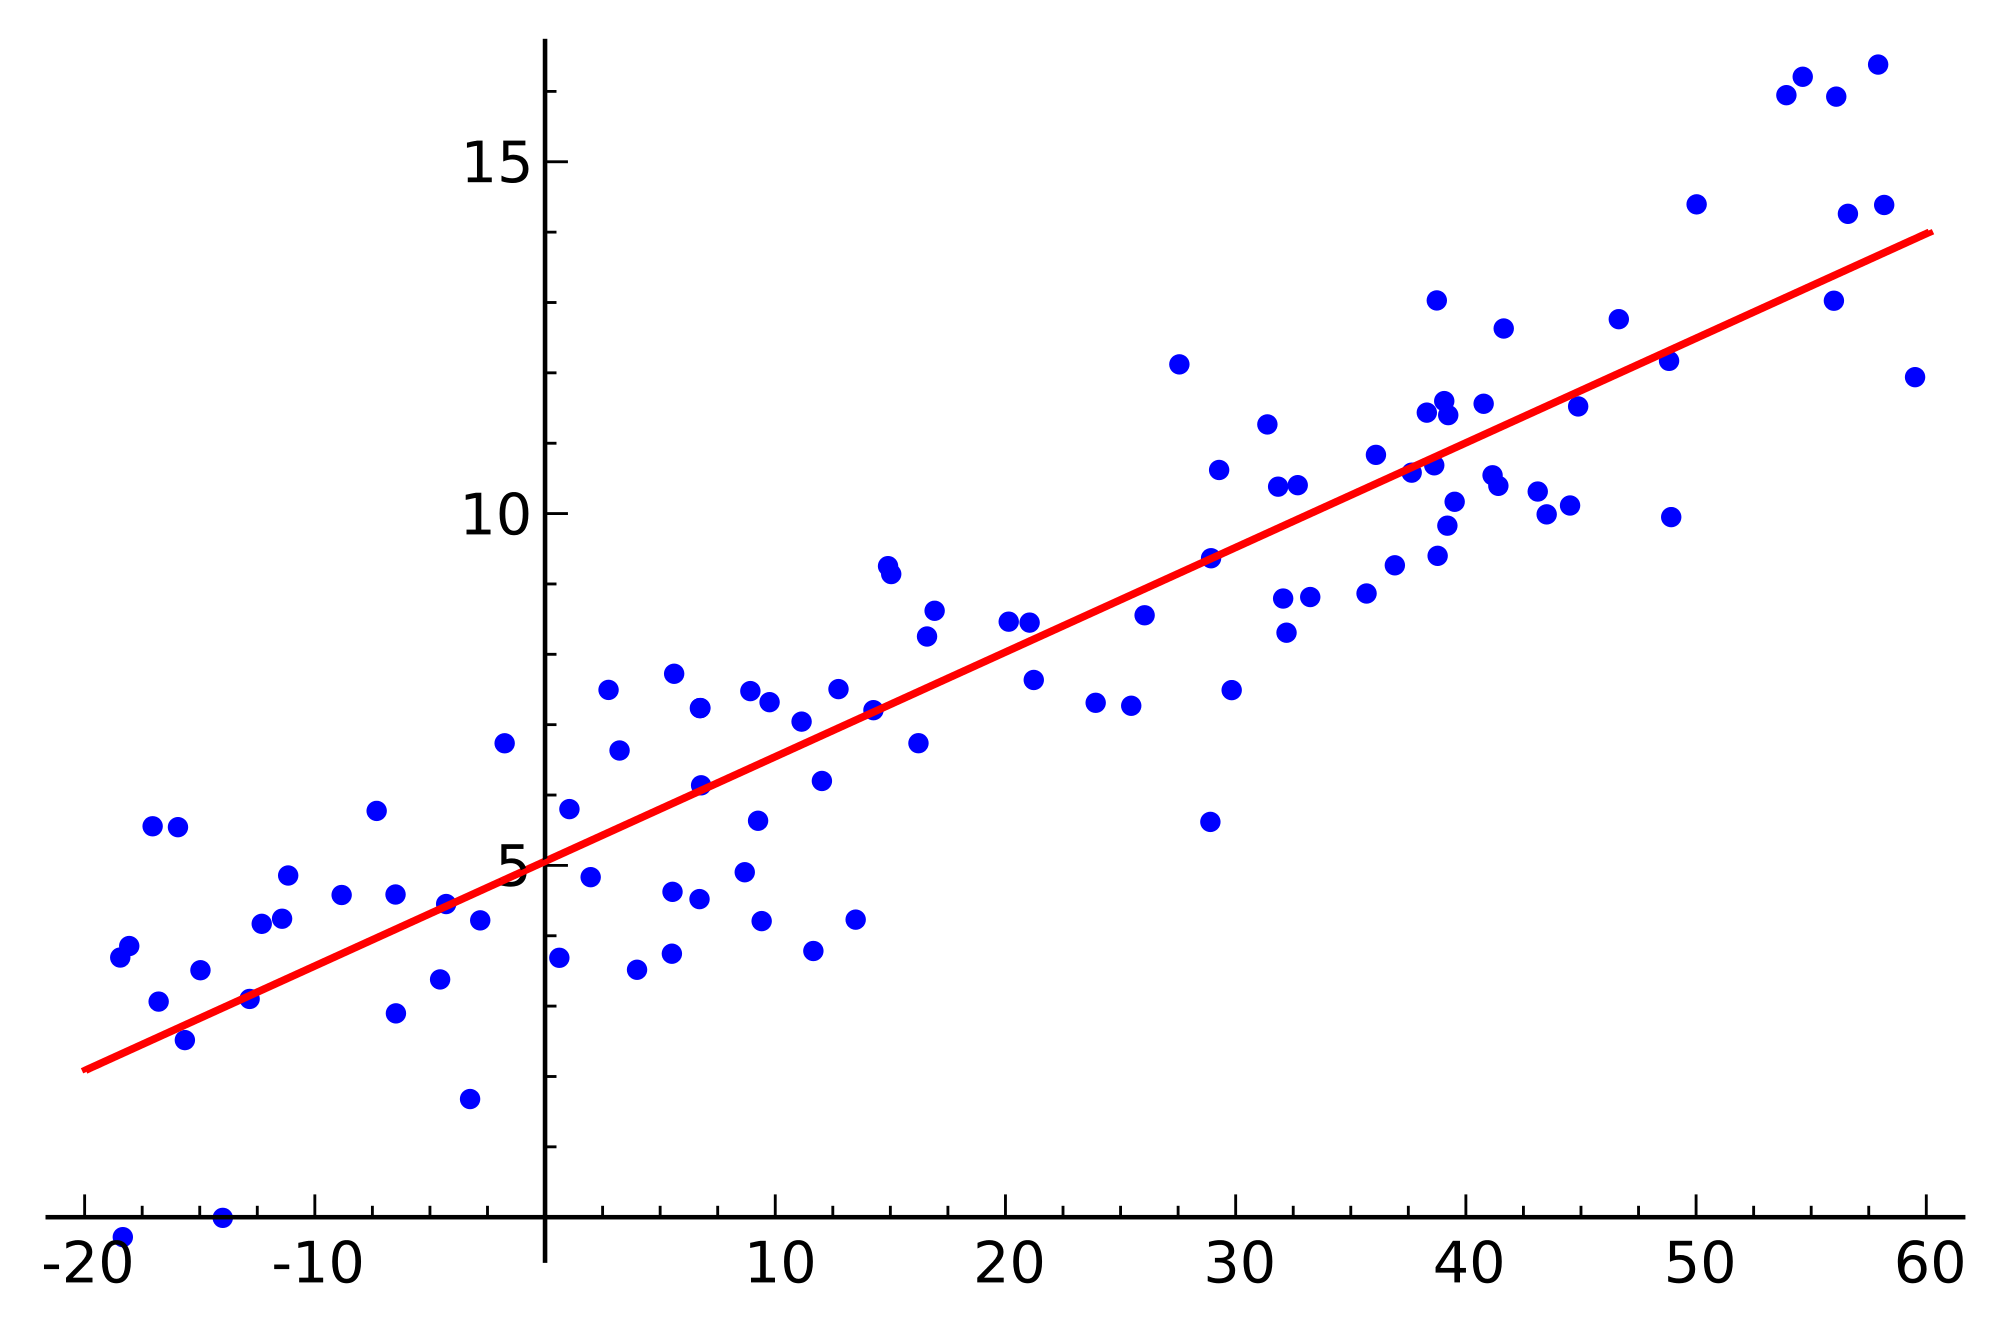
\includegraphics[width=0.6\textwidth]{Linear-regression}
	\caption{Example of simple linear regression with one variable}
	\label{fg:linear_regression}
\end{figure}


There are a large number of procedures which have been developed for parameters estimation and inference in linear regression. Spark MLlib uses least-square estimation\cite{7_mllib_linear_methods}.\\


Given a training set $ (x, y) $ (set number is $ n $), and initial weights $ w $, the error is computed as
\begin{equation}
error := \frac{1}{2} (w^T x - y)^2.
\label{eq:error_equation}
\end{equation}
This type of error is known as mean squared error (MSE).\\


After known the error, next step is using \emph{gradient descent} algorithm to update weight. Update equation is,
\begin{equation}
w_i=w_i-\alpha \frac{\partial}{\partial w_i} error
\label{eq:update_equation}
\end{equation}
Here $ \alpha $ is called learning rate. 


From above equation we can get that,
\begin{equation}
\begin{split}
\frac{\partial }{\partial w_i} error & = \frac{\partial }{\partial w_i} \frac{1}{2}(w^Tx-y)^2\\
& = 2 \cdot \frac{1}{2} (w^Tx-y) \cdot \frac{\partial }{\partial w_i} (w^Tx-y)\\
& = (w^Tx-y) * \frac{\partial }{\partial w_i} (\sum_{j=0}^{n}w_j x_j - y)\\
& = (w^Tx-y)x_i
\end{split}
\label{eq:partil_error}
\end{equation}


Then the updating rule becomes
\begin{equation}
w_i = w_i + \alpha (w^Tx-y)x_i
\end{equation}

This is gradient descent, also called batch gradient descent, the illustration is as figure~\ref{fg:gradient_descent}
\begin{figure}[h]
	\centering
	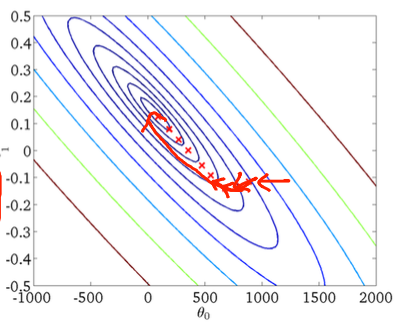
\includegraphics[width=0.6\textwidth]{steepest-descent}
	\caption{Illustration of gradient descent}
	\label{fg:gradient_descent}
\end{figure}

\clearpage
This algorithm runs very slow for a large data set input, as in every iteration, the errors of every data pair should be calculated.\\


Spark MLlib use \emph{stochastic gradient descent (SGD)} to speed up the training process\cite{7_mllib_linear_methods}.\\


The core idea of SGD is that updating parameters according to the gradient of the error with respect to that a small sample of training example (even one). The illustration of SGD can be found in figure~\ref{fg:SGD}
\begin{figure}[h]
	\centering
	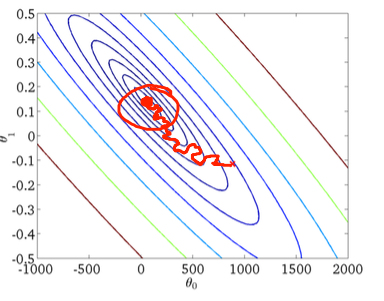
\includegraphics[width=0.6\textwidth]{sgd}
	\caption{Illustration of stochastic gradient descent (SGD)}
	\label{fg:SGD}
\end{figure}
Usually, SGD gets $ w $ "close" to the optimal solution more faster than batch gradient descent\cite{bottou2010large}, (but may never reach that solution), this makes SGD more suitable to large scale data regression.\\


In this study, the training iterations of our linear regression model are set to 100000, while the learning rate is 0.001.

\subsection{Random Forest}
